% This must be in the first 5 lines to tell arXiv to use pdfLaTeX, which is strongly recommended.
\pdfoutput=1
% In particular, the hyperref package requires pdfLaTeX in order to break URLs across lines.

\documentclass[11pt]{article}

% Change "review" to "final" to generate the final (sometimes called camera-ready) version.
% Change to "preprint" to generate a non-anonymous version with page numbers.
\usepackage[final]{acl}

% Standard package includes
\usepackage{times}
\usepackage{latexsym}
\usepackage{algorithmic}
\usepackage{graphicx}
\usepackage{textcomp}
\usepackage{xcolor}
\usepackage{physics}
\usepackage{mathdots}
\usepackage{algorithm}
\usepackage{subfigure}
\usepackage{pgfplots}
\usepackage{tikz}
\usetikzlibrary{patterns}
\usepackage{multirow}
\usepackage{multicol}
% \usepackage{authblk}
\usepackage{array}
\pgfplotsset{compat=1.18}

% 在这里添加这一行
\let\Bbbk\relax
\usepackage{amsmath,amssymb,amsfonts}
\DeclareMathOperator*{\argmax}{arg\,max}

% For proper rendering and hyphenation of words containing Latin characters (including in bib files)
\usepackage[T1]{fontenc}
% For Vietnamese characters
% \usepackage[T5]{fontenc}
% See https://www.latex-project.org/help/documentation/encguide.pdf for other character sets

% This assumes your files are encoded as UTF8
\usepackage[utf8]{inputenc}

% This is not strictly necessary, and may be commented out,
% but it will improve the layout of the manuscript,
% and will typically save some space.
\usepackage{microtype}

% This is also not strictly necessary, and may be commented out.
% However, it will improve the aesthetics of text in
% the typewriter font.
\usepackage{inconsolata}

%Including images in your LaTeX document requires adding
%additional package(s)
\usepackage{graphicx}

% If the title and author information does not fit in the area allocated, uncomment the following
%
%\setlength\titlebox{<dim>}
%
% and set <dim> to something 5cm or larger.

\title{Making RALM Robust to Irrelevant Contexts via Layer Knowledge Guided Attention}

% Author information can be set in various styles:
% For several authors from the same institution:
% \author{Author 1 \and ... \and Author n \\
%         Address line \\ ... \\ Address line}
% if the names do not fit well on one line use
%         Author 1 \\ {\bf Author 2} \\ ... \\ {\bf Author n} \\
% For authors from different institutions:
% \author{Author 1 \\ Address line \\  ... \\ Address line
%         \And  ... \And
%         Author n \\ Address line \\ ... \\ Address line}
% To start a separate ``row'' of authors use \AND, as in
% \author{Author 1 \\ Address line \\  ... \\ Address line
%         \AND
%         Author 2 \\ Address line \\ ... \\ Address line \And
%         Author 3 \\ Address line \\ ... \\ Address line}

\author{
 \textbf{Weijie Shi\textsuperscript{1}\thanks{Co-authors: Hao Chen, Yao Zhao}\thanks{\small{
   \textbf{Email:} \href{mailto:wshiah@connect.ust.hk}{wshiah@connect.ust.hk}
 }}},
 \textbf{Hao Chen\textsuperscript{2}\footnotemark[1]},
 \textbf{Jiaming Li\textsuperscript{2}},
 \textbf{Yao Zhao\textsuperscript{2}\footnotemark[1]},
\\
 \textbf{Yazhong Zhang\textsuperscript{2}\thanks{Corresponding authors: Yazhong Zhang, Qijin Chen, Jiajie Xu, Jia Zhu}},
 \textbf{Qijin Chen\textsuperscript{2}\footnotemark[3]},
 \textbf{Jipeng Zhang\textsuperscript{1}},
 \textbf{Ruiyuan Zhang\textsuperscript{1}},
\\
 \textbf{Jia Zhu\textsuperscript{3}\footnotemark[3]},
 \textbf{Jiajie Xu\textsuperscript{4}\footnotemark[3]},
 \textbf{Xiaofang Zhou\textsuperscript{1}}
\\
\\
 \textsuperscript{1}The Hong Kong University of Science and Technology,
 \textsuperscript{2}Alibaba Group, \\
 \textsuperscript{3}Zhejiang Key Laboratory of Intelligent Education Technology and Application, \\ Zhejiang Normal University,
 \textsuperscript{4}Soochow University
}
%\author{
%  \textbf{First Author\textsuperscript{1}},
%  \textbf{Second Author\textsuperscript{1,2}},
%  \textbf{Third T. Author\textsuperscript{1}},
%  \textbf{Fourth Author\textsuperscript{1}},
%\\
%  \textbf{Fifth Author\textsuperscript{1,2}},
%  \textbf{Sixth Author\textsuperscript{1}},
%  \textbf{Seventh Author\textsuperscript{1}},
%  \textbf{Eighth Author \textsuperscript{1,2,3,4}},
%\\
%  \textbf{Ninth Author\textsuperscript{1}},
%  \textbf{Tenth Author\textsuperscript{1}},
%  \textbf{Eleventh E. Author\textsuperscript{1,2,3,4,5}},
%  \textbf{Twelfth Author\textsuperscript{1}},
%\\
%  \textbf{Thirteenth Author\textsuperscript{3}},
%  \textbf{Fourteenth F. Author\textsuperscript{2,4}},
%  \textbf{Fifteenth Author\textsuperscript{1}},
%  \textbf{Sixteenth Author\textsuperscript{1}},
%\\
%  \textbf{Seventeenth S. Author\textsuperscript{4,5}},
%  \textbf{Eighteenth Author\textsuperscript{3,4}},
%  \textbf{Nineteenth N. Author\textsuperscript{2,5}},
%  \textbf{Twentieth Author\textsuperscript{1}}
%\\
%\\
%  \textsuperscript{1}Affiliation 1,
%  \textsuperscript{2}Affiliation 2,
%  \textsuperscript{3}Affiliation 3,
%  \textsuperscript{4}Affiliation 4,
%  \textsuperscript{5}Affiliation 5
%\\
%  \small{
%    \textbf{Correspondence:} \href{mailto:email@domain}{email@domain}
%  }
%}

\begin{document}
\maketitle
\begin{abstract}
Retrieval-augmented language models (RALMs) aim to incorporate external knowledge to address the issues of factual hallucination and knowledge obsolescence faced by large language models (LLMs). Inevitably, the retrieved passages based on similarity search may be irrelevant to the given question, and the aggregation of these passages can confuse the model to give a correct answer. To improve the performance of RALM in such conditions, we propose layer-knowledge guided attention for RALMs, which harnesses the layer-wise knowledge of LLMs to optimize per-layer attention on useful passages, making the model pay attention to the most relevant content and ignore irrelevant ones. Specifically, we first systematically study LLM's attention patterns and their relationship with the accuracy of RALM responses, where middle-focus attentions play a crucial role in selectively gathering relevant information. Based on this, a layer-wise passage estimator leverages the varied knowledge encoded across LLM layers to assess not only passage relevance scores but also associated confidences. Finally, a relevance-aware passage fusion enables selective attention to relevant passages, mitigating distractibility and positional bias of causal attention. Experiments show that our method outperforms existing methods on RALM benchmarks.
\end{abstract}

\section{Introduction}
Large language models (LLMs) have demonstrated remarkable performance, scalability, and adaptability in various natural language processing tasks \cite{bang2023multitask,guo2023close,chowdhery2022palm}. However, LLMs encounter significant challenges when tackling knowledge-intensive tasks, including factual hallucination \cite{cao2020factual,raunak2021curious,ji2023survey}, knowledge obsolescence \cite{he2022rethinking}, and a lack of domain-specific expertise \cite{shen2023chatgpt,li2023chatgpt}. To address these issues, retrieval-augmented language model (RALM) has emerged as a mainstream approach, which leverages a retrieval-then-read pipeline to supply external information for the LLM answering questions.

\begin{figure}[t]
\centering
\ref{combined_legend}
\subfigure[
Accuracy plateaus due to \textit{attention's distractibility}.
]{
\begin{minipage}[t]{0.45\linewidth}
\centering
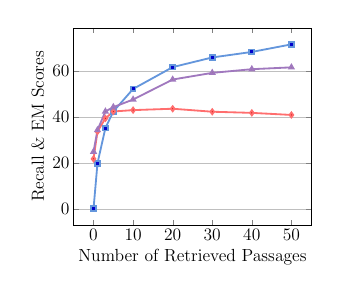
\begin{tikzpicture}[scale=0.44]
    \begin{axis}[
        xlabel=Number of Retrieved Passages,
        ylabel=Recall \& EM Scores,
        % y label style={at={(-0.00,0.5)}},
        ymajorgrids=true,
        font=\Large,
        legend style={at={(0.8,1.05)},anchor=south,legend columns=3,font={\fontsize{5pt}{5pt}\selectfont},/tikz/every even column/.append style={column sep=0.2cm}},
        legend to name=combined_legend
        ]
        \addplot+[color={rgb,255:red,100;green,150;blue,220},line width=1.5pt,mark=square*,mark size=2pt] coordinates {
            (0,0)
            (1,19.8)
            (3,35.1)
            (5,42.3)
            (10,52.1)
            (20,61.6)
            (30,65.8)
            (40,68.2)
            (50,71.5)
        };
        \addlegendentry{Retrieval Recall}
        \addplot+[color={rgb,255:red,255;green,110;blue,110},line width=1.5pt,mark=diamond*,mark size=2pt] coordinates {
            (0,21.7)
            (1,33.6)
            (3,39.3)
            (5,42.3)
            (10,42.9)
            (20,43.5)
            (30,42.2)
            (40,41.7)
            (50,40.8)
        };
        \addlegendentry{LLAMA with Retrieval}
        \addplot+[color={rgb,255:red,160;green,120;blue,190},line width=1.5pt,mark=triangle*,mark size=2pt] coordinates {
            (0,24.8)
            (1,34.2)
            (3,42.3)
            (5,44.2)
            (10,47.5)
            (20,56.2)
            (30,59.1)
            (40,60.7)
            (50,61.5)
        };
        \addlegendentry{LKG-RALM with Retrieval}
    \end{axis}
\end{tikzpicture}
\label{fig:retrieved passages number}
\end{minipage}
}
\hfill
\subfigure[U-shaped performance due to \textit{positional bias}.]{
\begin{minipage}[t]{0.45\linewidth}
\centering
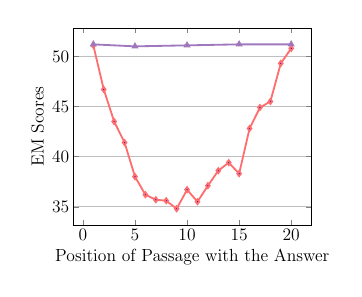
\begin{tikzpicture}[scale=0.44]
    \begin{axis}[
        xlabel=Position of Passage with the Answer,
        ylabel=EM Scores,
        % y label style={at={(-0.00,0.5)}},
        ymajorgrids=true,
        font=\Large,
        legend style={at={(0.5,1.05)},anchor=south,legend columns=3},
        legend cell align={left},
        ]
        \addplot+ [color={rgb,255:red,255;green,110;blue,110},line width=1.5pt,mark=diamond*,mark size=2pt] coordinates {
            (1,51.1)
            (2,46.7)
            (3,43.5)
            (4,41.4)
            (5,38.0)
            (6,36.2)
            (7,35.7)
            (8,35.6)
            (9,34.8)
            (10,36.7)
            (11,35.5)
            (12,37.1)
            (13,38.6)
            (14,39.4)
            (15,38.3)
            (16,42.8)
            (17,44.9)
            (18,45.5)
            (19,49.3)
            (20,50.8)
        };
        \addplot+ [color={rgb,255:red,160;green,120;blue,190},line width=1.5pt,mark=triangle*,mark size=2pt] coordinates {
            (1,51.2)
            (5,51.0)
            (10,51.1)
            (15,51.2)
            (20,51.2)
        };
    \end{axis}
\end{tikzpicture}
\label{fig:answer position}
\end{minipage}
}
\caption{Comparison of LLAMA's and LKG-RALM's performance with retrieved passages.}
\label{fig:LLM challenges}
\end{figure}

Despite RALM's potential, LLMs struggle to handle retrieved passages, which contain irrelevant ones, hindering performance in two aspects:
\begin{itemize}
    \item \textbf{Attention Distractibility}: As shown in Figure \ref{fig:retrieved passages number}, while increasing retrieved passages improves recall linearly, LLM accuracy plateaus or declines due to attention disruption from irrelevant content \cite{shi2023large}. The question tokens' attention becomes scattered across noisy information in the passages.
    \item \textbf{Positional Bias}: As  illustrated in Figure \ref{fig:answer position}, LLM performance exhibits a U-shaped curve based on passage position, with better handling of information at the start and end while missing crucial middle content \cite{liu2024lost}. This stems from LLM attention's over-reliance on positional information.
\end{itemize}
While RankRAG \cite{yoran2024making} attempts to address these issues by filtering irrelevant passages and optimizing passage placement, these serve as compromised strategies rather than fundamental fixes to LLM attention processing retrieved passages.

In this paper, we propose Layer-Knowledge Guided Attention for RALM (LKG-RALM), which harnesses the layer-wise knowledge of LLMs to optimize attention on useful passages. To effectively guide LLM's attention, accurately assessing the relevance of retrieved passages is crucial. Recent works demonstrate that LLM-based embeddings significantly outperform BERT-like models on the MTEB leaderboard due to superior scaling and comprehensive pre-training. Furthermore, \citet{rome,chuang2023dola} indicate that different LLM layers encode varied knowledge, from grammatical understanding in lower layers to reasoning capabilities in higher ones. Building on these insights, we propose a layer-wise passage estimator, which fully leverages varied knowledge of LLM layers to accurately predict both relevance and estimation confidence. Since not all layers' knowledge contributes equally to relevance assessment, an entropy-based layer-knowledge selection is proposed to dynamically determine which layers' knowledge is suitable for passages. To mitigate distractibility and positional bias from irrelevant passages, a relevance-aware passage fusion employs a relevance-guided attention mask to enable question tokens to selectively attend to retrieved passages for middle-focused attention patterns. Experiments demonstrate that LKG-RALM achieves substantial performance improvements across RALM datasets. Our contributions are summarized as:
\begin{itemize}
    \item We present the first systematic study on the relation between RALM's attention patterns and performance. Based on these, LKG-RALM leverages layer-wise knowledge to guide middle-focused attention toward relevant passages, thereby enhancing the understanding of retrieved information.
    \item We propose a layer-wise passage estimator to utilize LLM layer-specific knowledge to assess reliable and adaptable passage relevance.
    \item We propose relevance-aware passage fusion to enable question tokens to selectively attend to relevant passages, mitigating distractibility and positional bias.
\end{itemize}

\begin{figure*}[t]
\centering
\subfigure[Edge-focused Attention]{
    \begin{minipage}[t]{0.22\linewidth}
        \centering
        \includegraphics[width=0.95\linewidth]{figure/src/edge_focused_attention.pdf}
    \end{minipage}
    \label{fig:edge-focused}
}
\subfigure[Uniform Attention]{
    \begin{minipage}[t]{0.22\linewidth}
        \centering
        \includegraphics[width=0.95\linewidth]{figure/src/uniform_attention.pdf}
    \end{minipage}
    \label{fig:uniform}
}
\subfigure[Middle-focused Attention]{
    \begin{minipage}[t]{0.22\linewidth}
        \centering
        \includegraphics[width=0.95\linewidth]{figure/src/middle_focused_attention.pdf}
    \end{minipage}
    \label{fig:middle-focused}
}
\subfigure[Attention Distribution]{
    \begin{minipage}[t]{0.22\linewidth}
        \centering
        \includegraphics[width=0.9\linewidth]{figure/src/attention_distribution_pie.pdf}
    \end{minipage}
    \label{fig:distribution}
}
\caption{Attention patterns of RALM.}
\label{fig:attention pattern}
\end{figure*}
\begin{figure}[t]
\centering
\subfigure[Relation between attention pattern and RALM accuracy]{
    \begin{minipage}[t]{0.95\linewidth}
        \centering
        \includegraphics[width=\linewidth]{figure/src/ralm_accuracy_plot.pdf}
    \end{minipage}
    \label{fig:ralm-accuracy}
}
\subfigure[
Impact of replacing edge-focused and uniform attention with middle-focused attention on relevant passages]{
\begin{minipage}[t]{0.45\linewidth}
\centering
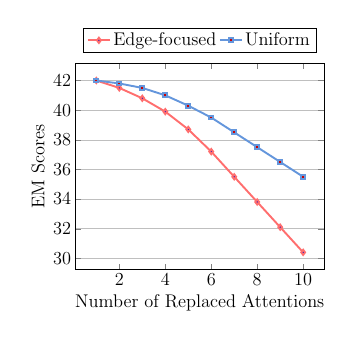
\begin{tikzpicture}[scale=0.46]
\begin{axis}[
xlabel=Number of Replaced Attentions,
ylabel=EM Scores,
% y label style={at={(-0.00,0.5)}},
ymajorgrids=true,
font=\Large,
legend style={at={(0.5,1.05)},anchor=south,legend columns=2},
% xmin=1, xmax=10,
]
\addplot+[color={rgb,255:red,255;green,110;blue,110},line width=1.5pt,mark=diamond*,mark size=2pt] coordinates {
(1,42.0)
(2,41.5)
(3,40.8)
(4,39.9)
(5,38.7)
(6,37.2)
(7,35.5)
(8,33.8)
(9,32.1)
(10,30.4)
};
\addlegendentry{Edge-focused}
\addplot+[color={rgb,255:red,100;green,150;blue,220},line width=1.5pt,mark=square*,mark size=1.5pt] coordinates {
(1,42.0)
(2,41.8)
(3,41.5)
(4,41.0)
(5,40.3)
(6,39.5)
(7,38.5)
(8,37.5)
(9,36.5)
(10,35.5)
};
\addlegendentry{Uniform}
\end{axis}
\end{tikzpicture}
\label{fig:attention replacement}
\end{minipage}
}
\hfill
\subfigure[
Impact of manipulating middle-focused attention patterns on relevant passages
]{
\begin{minipage}[t]{0.45\linewidth}
\centering
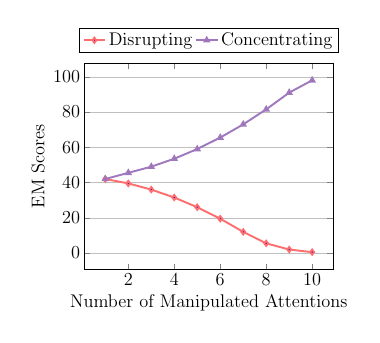
\begin{tikzpicture}[scale=0.46]
\begin{axis}[
xlabel=Number of Manipulated Attentions,
ylabel=EM Scores,
% y label style={at={(-0.00,0.5)}},
ymajorgrids=true,
font=\Large,
legend style={at={(0.5,1.05)},anchor=south,legend columns=2},
legend cell align={left},
% xmin=1, xmax=10,
]
\addplot+[color={rgb,255:red,255;green,110;blue,110},line width=1.5pt,mark=diamond*,mark size=2pt] coordinates {
(1,42.0)
(2,39.5)
(3,36.0)
(4,31.5)
(5,26.0)
(6,19.5)
(7,12.0)
(8,5.5)
(9,2.0)
(10,0.5)
};
\addlegendentry{Disrupting}
\addplot+ [color={rgb,255:red,160;green,120;blue,190},line width=1.5pt,mark=triangle*,mark size=2pt] coordinates {
(1,42.0)
(2,45.5)
(3,49.0)
(4,53.5)
(5,59.0)
(6,65.5)
(7,73.0)
(8,81.5)
(9,91.0)
(10,98.0)
};
\addlegendentry{Concentrating}
\end{axis}
\end{tikzpicture}
\label{fig:attention manipulation}
\end{minipage}
}
\caption{Impact of manipulating attention patterns on RALM performance.}
\label{fig:attention evidence}
\vspace{-0.5cm}
\end{figure}

\section{Related Work}
\subsection{Retrieval-augmented Language Model}
Retrieval-augmented language models (RALMs) \cite{survey1,zhao2023survey,survey2} enhance generation by incorporating retrieved passages through three main approaches: query-based fusion, which concatenates passages with input queries \cite{REPLUG,RALM} or features \cite{FID,liu2023recap}; logits-based fusion, which combines probability distributions from input and retrieved passages \cite{khandelwal2019generalization,huang2023k}; and latent fusion, which integrates passages into hidden states via attention \cite{wang2023shall} or weighted additions \cite{wu2024improving}.

Recent work has focused on addressing noise in retrieved passages. \citet{liu2024lost} analyzed position bias across model types and query positions, while \citet{shi2023large,wu2024instructing} attempted to incorporate passage relevance into context. Other approaches include filtering irrelevant passages \cite{zhang2021drop,yoran2024making} and developing noise-resistant fine-tuning strategies \cite{liu2024chatqa,yu2024rankrag}. However, these methods remain constrained by reranking accuracy and fail to address the fundamental limitations of causal attention. Our work investigates the relationship between attention patterns and RALM performance, leading to our LKG-RALM approach that leverages layer-wise knowledge for improved passage attention.

\subsection{Passage Relevance Assessment}
While traditional methods like BM25 \cite{bm25} and BERT-based models \cite{DPR,contriever,bge} have advanced text representation, they face scaling challenges in representation training. Recent approaches \cite{wang2023improving,behnamghader2024llm2vec,springer2024repetition} have shown promise in adapting decoder-only LLMs as text encoders through contrastive learning. However, even state-of-the-art models achieve only 62\% accuracy on the MTEB leaderboard \cite{MTEB}, highlighting the need for more nuanced relevance assessment approaches. 

\citet{rome,chuang2023dola,zhang2024comprehensive} have shown that LLMs encode layer-specific knowledge, ranging from grammatical structures in lower layers to complex reasoning in higher ones. Building on this insight, we propose a layer-wise passage estimator that leverages this hierarchical knowledge structure to provide comprehensive relevance assessments with reliability measures.



\begin{figure*}[t]
\centering
\begin{minipage}[t]{1\linewidth}
\centering
\includegraphics[width=1.03\textwidth]{figure/src/llm framework.pdf}
\end{minipage}
\centering
\caption{The architectures of LKG-RALM.}
\label{fig:llm framework}
\end{figure*}

\section{Preliminaries}
\subsection{Problem Formalization}
Our method is depicted under the open question-answering (open-QA) settings, aiming to predict an answer $y_{ans}$ based on a question $q$ and $n$ retrieved passages $[p_1,\dots,p_n]$. 

\subsection{Analysis of Attention Patterns of RALM}
To address the challenges of attention's distractibility and positional bias in RALM, it is crucial to systematically investigate its attention patterns. The attention mechanism selects specific tokens to gather information from retrieved passages for the generation of next token. Following the \citet{fu2024attentionpattern} methodology, we conducted a systematic study on the attention distribution of LLAMA-3.1-8B using 2000 samples from the NQ and TriviaQA dataset (details in Appendix \ref{Attention pattern analysis}). Figure \ref{fig:attention pattern} reveals three distinct attention patterns that potentially impact the model's ability to process retrieved passages.


\textbf{Edge-focused attention}, observed in 78\% of attention heads, shows over 99\% of attention concentrating on the beginning and end of the context. \citet{xiao2023efficient} demonstrated that this phenomenon persists even when replacing the initial tokens with meaningless ones, indicating that the model emphasizes absolute position rather than semantic value. This pattern correlates strongly with positional bias, hindering the model's ability to process crucial information in the middle of the input sequence.

\textbf{Uniform attention}, accounting for 5.37\% of patterns, distributes attention almost uniformly across all tokens in the context. While appearing to provide equal consideration to all information, this pattern potentially contributes to the model's distractibility by failing to focus on the most relevant parts of the input.

\textbf{Middle-focused attention}, though present in only 6\% of attention heads, manifests in two variants: "scattered over middle" and "concentrated on middle". The former distributes attention across several tokens, while the latter concentrates on only one or two tokens. This pattern plays a crucial role in selectively gathering information from the context, essential for comprehending retrieved passages.

To analyze the relationship between these patterns and RALM performance, we examined the correlation between attention weight sums and model accuracy. Figure \ref{fig:attention pattern}(d) reveals that increased attention on relevant passages in edge-focused and uniform patterns yielded no performance gains, while middle-focused patterns demonstrated a strong positive correlation with RALM accuracy. Manipulation experiments further supported these findings: artificially replacing edge-focused and uniform patterns with middle-focused attention on relevant passages disrupted the model's attention structure, leading to performance degradation. As shown in Figure \ref{fig:attention manipulation}, deliberately redirecting middle-focused patterns to irrelevant passages significantly decreased performance, while concentrating this attention on relevant passages improved it. These results suggest that guiding middle-focused attention towards relevant passages could significantly enhance RALM's effectiveness.

% \begin{figure}[t]
\centering
\begin{minipage}[t]{1\linewidth}
\centering
\includegraphics[width=1.0\textwidth]{figure/src/OQDApipeline.pdf}
\end{minipage}
\centering
\caption{Comparison between naive passage concatenation (right) and relevance-aware passage integration (left) in RALM. Due to low retrieval accuracy, the LLM is distracted by a vast number of \textcolor{red!80!black}{noisy tokens}. In contrast, explicitly guiding the LLM's attention to more \textcolor{green!60!black}{relevant passages} can effectively enhance its comprehension.}
\label{fig:llm pipeline}
\end{figure}

\begin{figure}[t]
\centering
\begin{minipage}[t]{1\linewidth}
\centering
\includegraphics[width=0.95\textwidth]{figure/src/Passage Relevance Estimator.pdf}
\end{minipage}
\centering
\caption{The layer-wise passage estimator.}
\label{fig:passage relevance estimator}
\end{figure}

\section{Methodology}
\subsection{Overview}
The vanilla attention of LLMs often suffers from distractibility and positional bias, which is unsuitable for open-QA with retrieved passages. We take advantage of layer-wise knowledge of LLMs to assess passage relevance, then guide the LLM's attention to generate answers, effectively mitigating these issues. The overall framework is illustrated in Figure \ref{fig:llm framework}.

% It first utilizes a layer-wise passage estimator to mine diverse knowledge encoded in different LLM layers, assessing the relevance of retrieved passages along with the reliability and adaptability of these relevance scores. Next, these assessments guide the LLM's attention through a relevance-aware passage integration component, enhancing robustness against irrelevant passages. Finally, three tailored losses optimize the relevance estimations, while a language model loss jointly fine-tunes the estimator and the LLM for improved performance.

\subsection{Adding Special Tokens}
To clearly delineate the boundary of the given question and each passage, we introduce trainable special tokens into the sequence. Specifically, we add \textcolor{blue}{$[d]$} and \textcolor{orange}{$[e_i]$} tokens as boundary markers at the beginning and end of each retrieved passage, respectively, while \textcolor{blue}{$[q]$} and \textcolor{yellow!70!black}{$[e_q]$} tokens demarcate the question.

\subsection{Layer-wise Passage Estimator}
Traditional passage estimators often rely on BERT-like structures, but these methods typically yield low accuracy and fail to leverage the rich, layer-specific knowledge embedded in LLMs. We propose a layer-wise passage estimator as Figure \ref{fig:passage relevance estimator}, which utilizes per-layer knowledge of LLM to assess relevance scores from multifaceted views, along with their associated confidence. Additionally, it incorporates an entropy-based layer-knowledge selection, which analyzes the attention distribution to determine the applicability of each layer's knowledge to the passages. By combining these comprehensive estimations, our approach provides trustworthy guidance for the LLM's attention.

\subsubsection{Layer-wise Relevance and Confidence Estimation.}
For a given layer $l$, we leverage the LLM's internal representations to compute relevance and confidence scores.  To adapt the LLM's parameter to relevance assessment, we add trainable low-rank weights (LoRA) to each decoder layer. To enhance contextual understanding within passages, we follow previous work \cite{behnamghader2024llm2vec} to adopt Blocked Bidirectional Attention Mask rather than the causal attention. To aggregate sentence-level information, we extract the hidden states of the last special tokens as sentence embedding: $e_i$ for each passage and $e_q$ for question. An adapter and dropout components are then used to enhance their robustness. Finally, two cross-attention components compute the relevance scores $r_1,\dots,r_n$ and confidence scores $c_1,\dots,c_n$ between passages and the question, respectively.

\subsubsection{Optimizing Estimator.}
To optimize our layer-wise passage estimator, we introduce three specialized loss functions, each addressing a crucial aspect of effective relevance estimation:

\paragraph{Relevance Loss.} To ensure the model accurately identifies relevant passages, we employ a relevance loss. This loss function encourages the estimated relevance scores to closely align with the ground truth, thereby improving the model's ability to distinguish between relevant and irrelevant passages:
\begin{equation}
L_{relevance} = -\frac{1}{n} \sum_{i=1}^n [\bar{r_i} \log(r_i) + (1-\bar{r_i}) \log(1-r_i)]
\end{equation}
where $\bar{r_i}$ is the ground truth label, and $r_i$ is the estimated relevance score. 

\paragraph{Confidence Loss} Recognizing that not all relevance predictions are equally reliable, we introduce a confidence loss. We posit that the model should exhibit high confidence for easier samples to classify, while maintaining lower confidence for more challenging and confusing cases. To this end, we leverage external models (such as BGE \cite{bge}) to assist in determining sample difficulty:
\begin{equation}
L_{confidence}\!\! =\!\! -\!\!\sum_{i=1}^n\! ( c_i \!  - \! [ \!\frac{1}{K} \!\! \sum_{k=1}^K I(M_k(r_i|q) \!\! == \! \bar{r_i})])
\end{equation}
where $c_i$ is the estimated confidence score, $M_k$ represents $K$ different external models, and $I(\cdot)$ is the indicator function. This loss trains the model to produce confidence scores that accurately reflect the trustworthiness of its relevance predictions:

\paragraph{Diversity Loss.} To ensure a comprehensive utilization of layer-specific knowledge and avoid overly homogeneous relevance guidance, we employ a diversity loss based on the entropy of the final relevance guidance:
\begin{equation}
L_{diversity} = -H(\alpha_1, \ldots, \alpha_n)
\end{equation}
where $H(\cdot)$ is the entropy function, and $\alpha_1, \ldots, \alpha_n$ are the final relevance guidance weights.

Combining these loss functions through simple addition, our estimator learns to provide accurate, confident, and diverse relevance assessments across different layers of the LLM. The Relevance Loss helps to quickly narrow down the search space to the most pertinent passages, while the Diversity Loss encourages a broader exploration of potentially relevant information, increasing the chances of recalling the correct answer. Although these two losses may seem antagonistic, their balanced combination leads to a more robust and comprehensive relevance assessment. 

\subsubsection{Entropy-based Layer-Knowledge Selection.}
Inspired by \citet{hyeon2023scratching}, to ensure the effective utilization of layer-specific knowledge in passage assessment, we propose an entropy-based layer-knowledge selection to identify which layers provide the most informative and contextually rich representations for each passage.

Specifically, for each passage $p_i$, we calculate the entropy $H_i$ of the attention distribution from each passage's last special token to other tokens in the sequence:
\begin{equation}
H_i = -K\sum_{j=1}^{n} w_i^j \log w_i^j
\end{equation}
where $w_i^j$ denotes the attention weight from the last special token $e_i$ to the $j$-th token in the sequence, $n$ is token number of passage $p_i$, and $K$ is the scaling factor. A higher entropy value indicates that the sentence embedding gathers a broader range of contextual information.

Finally, we use a selection weight to aggregate the layer-wise relevance and confidence scores to update the relevance guidance:
\begin{equation}
\begin{aligned}
\alpha_i^l = \beta &\left(\log(1 + H_i) \cdot \log(1 + r_i) \cdot \log(1 + c_i)\right) \\
                   &+ (1-\beta) \alpha_i^{l-1}
\end{aligned}
\end{equation}
where $\alpha_i^l$ is the updated relevance guidance for passage $p_i$ at layer $l$, and $\beta$ balances current and previous layer assessments. To mitigate numerical oversensitivity, we employ a logarithmic multiplication. This approach combines layer-wise relevance and confidence estimation with entropy-based layer-knowledge selection, enabling our estimator to leverage diverse knowledge across LLM layers and provide robust guidance for the LLM's attention mechanism. 

\subsection{Relevance-aware Passage Fusion}
To mitigate the issues of distractibility and positional bias, we propose a Relevance-aware Passage Fusion that selectively directs LLM attention to relevant passages based on the relevance guidance obtained from the Layer-wise Passage Estimator.

To effectively guide the LLM's attention towards relevant passages while mitigating the effects of distractibility and positional bias inherent in traditional attention frameworks, we introduce a relevance-guided attention mask. This mask dynamically modulates query-passage interactions based on estimated relevance, preserves intra-passage context, and inhibits cross-passage interference, thereby enhancing the model's capacity to prioritize salient information. The mask modulates the attention weights based on the estimated relevance of each passage. Formally, for each layer $l$, we define the attention mask $M^l$ as:
\begin{equation}
M^l_{ij} = \begin{cases}
\begin{aligned}
&\alpha_k^l, & &\text{if } i \in q \text{ and } j \in p_k \\
& & &\text{(middle-focused attention heads)} \\
&1, & &\text{if } i \in q \text{ and } j \in p_k \\
& & &\text{(other attention heads)} \\
&1, & &\text{if } i \in p_k \text{ and } j \in p_k \\
& & &\text{(same passage)} \\
&0, & &\text{if } i \in p_k \text{ and } j \in p_m \text{ where } k \neq m \\
& & &\text{(different passages)}
\end{aligned}
\end{cases}
\end{equation}
where $q$ represents the set of query token positions, $p_k$ is the set of token positions for passage $k$, and $\alpha_k^l$ is the relevance guidance for passage $k$ at layer $l$. As our analysis of RALM attention, we selectively apply relevance-guided attention mask to Middle-focused attention heads only, while maintaining the functionality of Edge-focused and Uniform attention patterns. Finally, we use the standard language modeling loss to jointly fine-tune the LLM. 

\section{Experiments}
\subsection{Experimental Setting}
\subsubsection{Datasets}
To assess performance across diverse data characteristics, we employ a range of representative datasets for RALM evaluation. These include Natural Question (NQ) \cite{NQ}, TriviaQA \cite{TQA}, StrategyQA \cite{strategyQA}, HotpotQA \cite{HotpotQA}, PopQA \cite{PopQA}, and 2WikiMQA \cite{ho2020constructing}. Detailed descriptions are provided in Appendix \ref{dataset description}.

\subsubsection{Baselines}
We categorize our baselines into three groups: closed-book LLM without retrieval, LLM with retrieval, and robust RALM. The first two groups include LLAMA-3.1 \cite{dubey2024llama}, Qwen-2.5 \cite{yang2024qwen2}, ChatGPT, GPT4, and Claude-3-Sonnet. The third group comprises REPLUGE \cite{REPLUG}, Self-RAG \cite{asai2023self}, RA-ISF \cite{liu2024ra} Noise-Resistant \cite{yoran2024making}, ChatQA-1.5 \cite{liu2024chatqa} and RankRAG \cite{yu2024rankrag}. Comprehensive descriptions of these baselines are provided in Appendix \ref{baseline setting}.

\subsubsection{Evaluation criteria}
In evaluating the quality of the predicted answers, we employ the standard exact match (EM) metric on 5-shot, following previous work \cite{DPR,atlas}. The generated answer is first normalized by lowercasing, removing articles, punctuation, and duplicated whitespace. The EM score is binary for one question, with a value of 1 if the predicted answer matches the ground-truth answer exactly, and 0 otherwise. Then we averaged the EM scores across all questions in the test set and then multiplied by 100 to obtain final scores.

\subsection{Overall Performance}
\setlength{\tabcolsep}{3.2pt}  % 默认值是6pt
\begin{table}[t]
\scriptsize
\begin{center}
\caption{Overall Performance. \textbf{Bold} numbers indicate the best score across all models, while underlined numbers represent the best score within each category.}
\begin{tabular}{lccccc} 
\hline
\textbf{Model} & \textbf{NQ} & \textbf{TriviaQA} & \textbf{HotpotQA} & \textbf{PopQA} & \textbf{2WikiMQA} \\
\hline
\multicolumn{6}{c}{\textit{General LLMs}} \\
LLAMA-3.1-8B & 18.7 & 78.5 & 16.5 & 22.1 & 13.9 \\
\quad + Retrieval & 30.9 & 70.7 & 26.0 & 34.9 & 9.6 \\ 
\quad + Fine-tuning & 35.7 & 77.4 & 28.9 & 37.1	& 25.3 \\ 
LLAMA-3.1-70B & 21.8 & 89.7 & 24.1 & 27.5 & 21.6 \\
\quad + Retrieval & 42.7 & 82.4 & 35.5 & 45.3 & 13.5 \\
\quad + Fine-tuning & 44.9 & 89.1 & 38.5 & 50.3 & 28.4 \\ 
Qwen-2.5-7B & 37.5 & 80.2 & 20.3 & 24.8 & 16.2 \\
\quad + Retrieval & 44.3 & 83.5 & 29.7 & 37.8 & 17.8 \\
\quad + Fine-tuning & 46.1 & 86.3 & 30.8 & 40.6 & 28.8 \\ 
Qwen-2.5-72B & 39.9 & 90.5 & 26.3 & 29.8 & 24.1 \\
\quad + Retrieval & 45.1 & 90.6 & 37.2 & 47.9 & 27.7 \\
\quad + Fine-tuning & 47.6 & 90.5 & \underline{39.4} & 52.2 & \underline{36.0} \\ 
ChatGPT & 38.6 & 82.9 & 29.9 & 28.4 & 23.9 \\ 
\quad + Retrieval & 46.7 & 79.7 & 31.2 & 49.9 & 27.2 \\ 
GPT-4 & 40.3 & 87.0 & 34.5 & 31.3 & 29.8 \\ 
\quad + Retrieval & 40.4 & 75.0 & 27.6 & 44.3 & 14.4 \\ 
Claude-3-Sonnet & 49.2 & 87.5 & 32.8 & 33.4 & 31.4 \\ 
\quad + Retrieval & \underline{55.1} & \textbf{90.8} & 33.3 & \underline{52.4} & 32.6 \\ 
\hline
\multicolumn{6}{c}{\textit{Robust RALM}} \\
REPLUGE & 23.8 & 58.6 & 21.8 & 40.1 & 25.7 \\ 
Self-RAG & 28.4 & 61.6 & 25.4 & 44.8 & 30.2 \\ 
RA-ISF & 31.3 & 63.2 & 28.9 & 46.8 & 31.7 \\ 
Noise-Resistant RALM & 45.7 & 80.3 & 34.4 & 48.1 & 34.7 \\ 
ChatQA-1.5 & 47.0 & 85.6 & 35.5 & 45.3 & 13.5 \\ 
RankRAG & \underline{54.2} & \underline{86.5} & \underline{42.7} & \underline{59.9} & \underline{38.2} \\ 
\hline
\multicolumn{6}{c}{\textit{LKG-RALM}} \\
LLAMA-3-8B & 53.6 & 87.9 & 42.4 & 56.5 & 38.7 \\ 
LLAMA-3-70B & 59.9 & 89.5 & 44.7 & 62.0 & 41.1 \\ 
LLAMA-3.1-8B & 55.3 & 88.6 & 43.1 & 57.2 & 39.0 \\ 
LLAMA-3.1-70B & 61.0 & 89.9 & 45.8 & 62.6 & 41.3 \\ 
Qwen-2.5-7B & 55.4 & 88.1 & 43.1 & 57.4 & 39.7 \\
Qwen-2.5-72B & \textbf{61.5} & \underline{90.0} & \textbf{46.1} & \textbf{62.7} & \textbf{41.4} \\
\hline
\end{tabular}
\label{table:overall performance}
\end{center}
\end{table}


The results in Table 1 demonstrate varying performance across different model types. Closed-book LLMs show strong baseline performance but face limitations in their knowledge base. Adding retrieval generally improves performance, as seen with LLAMA-3.1-70B improving from 21.8 to 42.7 on NQ, and further fine-tuning brings additional gains (reaching 44.9). However, this improvement isn't consistent across all models and datasets. For instance, GPT-4 with retrieval shows decreased performance on TriviaQA (87.0 to 75.0).

The combination of retrieval and fine-tuning shows promising results, particularly for larger models. Qwen-2.5-72B benefits significantly from both enhancements, with performance on NQ improving from 39.9 (base) to 45.1 (+ retrieval) to 47.6 (+ retrieval \& fine-tuning). Claude-3-Sonnet with retrieval achieves strong results, reaching 55.1 on NQ and 90.8 on TriviaQA. Robust RALM methods, particularly RankRAG, demonstrate effective utilization of retrieved passages, showing consistent improvements across datasets. RankRAG achieves strong performance with 54.2 on NQ and 59.9 on PopQA, outperforming many traditional retrieval-augmented approaches.

LKG-RALM outperforms baseline models across all datasets. Compared to closed-book LLMs, it shows substantial gains of 12.3 percentage points on NQ to 10.0 on 2WikiMQA. When compared to retrieval-augmented and fine-tuned models, LKG-RALM still demonstrates superior performance, with Qwen-2.5-72B based LKG-RALM achieving the best results across most metrics (61.5 on NQ, 46.1 on HotpotQA). The performance gap between 8B and 70B variants (2.3-5.7 percentage points) suggests that larger models can better leverage our approach, particularly on complex tasks like PopQA.


\subsection{Ablation Results}
\setlength{\tabcolsep}{3.2pt}  % 默认值是6pt
\begin{table}[t]
\begin{center}
\scriptsize
\caption{Ablation result of LKG-RALM, where "LPR", "ELS", and "RPF" stand for Layer-wised Passage Relevance, Entropy-based Layer-Knowledge Selection, and Relevance-aware Passage Fusion, respectively.}
\begin{tabular}{lccccc} 
\hline
\textbf{Model Varient} &  \textbf{NQ}  &  \textbf{TriviaQA} & \textbf{HotpotQA} & \textbf{PopQA} & \textbf{2WikiMQA} \\ 
\hline 
LKG-RALM-8B   &  55.3  & 88.6 & 43.1 & 57.2 & 39.0  \\
\hline
w/o LPR & 50.6  & 86.0 & 39.5 & 52.5 & 34.8  \\
w/o ELS &  53.1  & 87.7 & 41.8 & 55.8 & 37.2  \\
w/o RPF  & 30.9  & 70.7 & 26.0 & 34.9 & 9.6  \\
w/o Auxiliary Loss  & 54.2  & 87.3  & 42.3 & 56.4 & 37.8  \\
\hline
\end{tabular}
\label{table:q2-2}
\end{center}
\end{table}
\subsubsection{Effect of Designed Components}
Table \ref{table:q2-2} shows the ablation results of LKG-RALM with LLAMA-3.1-8B as the backbone. All proposed components contribute significantly to the final performance. Replacing the Layer-wise Passage Estimator with a reranking model causes a substantial performance drop across all tasks, with an average decrease of 3.96. This highlights its crucial role in using layer-wised LLM knowledge to assess passage relevance. The Entropy-based Layer-Knowledge Selection mechanism proves effective, as its removal leads to an average EM decrease of 1.52, showing the importance of dynamically selecting informative layer representations for each passage. Ablating the Relevance-aware Passage Fusion component results in significant performance degradation, with an average EM decrease of 22.22. This demonstrates our approach's effectiveness in reducing distractibility and positional bias when processing multiple passages, compared to traditional attention mechanisms. Finally, the auxiliary losses improve performance across most tasks by 1.06, indicating their value in guiding the model to consider passage relevance, prediction confidence, and diverse utilization of layer knowledge during training.

% Table \ref{table:q2-2} presents the ablation results of LKG-RALM with LLAMA-3.1-8B as the backbone. Overall, we observe that all of the proposed components contribute significantly to the final performance. Replacing the Layer-wise Passage Estimator with a reranking model leads to a substantial performance drop across all tasks, with an average decrease of 3.96. This underscores its crucial role in utilizing layer-wised LLM knowledge to assess the relevance of retrieved passages. Besides, the Entropy-based Layer-Knowledge Selection mechanism also proves to be effective, as its removal leads to an average EM decrease of 1.52, highlighting the importance of dynamically selecting the most informative layer representations for each passage. Ablating the Relevance-aware Passage Fusion component causes significant performance degradation, with an average EM decrease of 22.22. This demonstrates the effectiveness of our approach in mitigating distractibility and positional bias when processing multiple passages, compared to traditional attention mechanisms. Finally, the auxiliary losses contribute to improved performance across most tasks by 1.06, indicating their value in guiding the model to explicitly consider passage relevance, prediction confidence, and diverse utilization of layer knowledge during training.

\subsection{Robustness Analysis}
\subsubsection{Increased Number of Retrieved Passages}
To assess the scalability and efficiency of LKG-RALM in handling larger amounts of retrieved information, we conducted experiments varying the number of retrieved passages from 0 to 50. Figure \ref{fig:q4-1} illustrates the performance trends of LKG-RALM compared to baseline models across different datasets.

The experiment reveals that LKG-RALM demonstrates superior scalability and maintains high performance even as the number of retrieved passages increases significantly. LKG-RALM shows a steady increase in EM scores from 24.8 to 61.5 as the number of passages grows, with only a slight plateau effect beyond 35 passages, indicating effective utilization of additional information without suffering from information overload. In contrast, baseline models like RankRAG and Self-RAG initially show improvements with more passages, but their performance begins to degrade or plateau beyond 25 passages. RankRAG reaches a peak of 53.7 at 25 passages before slightly declining to 54.2 at 50 passages, while Self-RAG peaks at 43.5 at 25 passages before sharply declining to 28.4 at 50 passages. GPT-4 with Retrieval shows remarkable stability, maintaining a nearly constant performance (around 40.4) regardless of the number of passages, indicating its strong innate knowledge but potential limitations in effectively utilizing additional retrieved information. 

LKG-RALM maintains its edge, with a 6.8 EM score advantage over RankRAG at 50 passages (61.0 vs 54.2). Despite the increased potential for irrelevant information with more passages, LKG-RALM's performance remains robust, underscoring the effectiveness of its relevance-aware passage fusion mechanism. 

\subsubsection{Higher Proportions of Irrelevant Passages}
\begin{figure}[t]
\centering
\subfigure[Impact of Increasing Passage Number]{
\begin{minipage}[t]{0.45\linewidth}
\centering
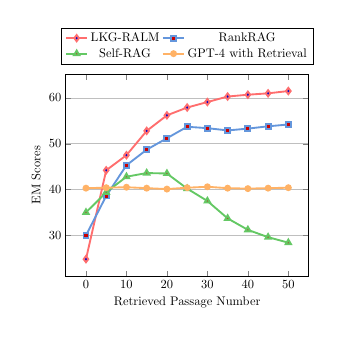
\begin{tikzpicture}[scale=0.45]
    \begin{axis}[
        xlabel=Retrieved Passage Number,
        ylabel=EM Scores,
        % y label style={at={(-0.0,0.5)}},
        ymajorgrids=true,
        font=\Large,
        legend style={at={(0.5,1.05)}, anchor=south, legend columns=2, draw=black, fill=white,align=left},font=\normalsize
    ]
        \addplot+[color={rgb,255:red,255;green,110;blue,110}, line width=1.5pt, mark=diamond*, mark size=2.5pt] coordinates {        
            (0,24.8)
            (5,44.2)
            (10,47.5)
            (15,52.8)
            (20,56.2)
            (25,57.9)
            (30,59.1)
            (35,60.3)
            (40,60.7)
            (45,61.0)
            (50,61.5)
        };
        \addlegendentry{LKG-RALM};
        \addplot+[color={rgb,255:red,100;green,150;blue,220}, line width=1.5pt, mark=square*, mark size=2pt] coordinates {
            (0,30.0)
            (5,38.6)
            (10,45.3)
            (15,48.7)
            (20,51.2)
            (25,53.7)
            (30,53.4)
            (35,52.9)
            (40,53.3)
            (45,53.8)
            (50,54.2)
        };
        \addlegendentry{RankRAG};
        \addplot+[color={rgb,255:red,100;green,200;blue,100}, line width=1.5pt, mark=triangle*, mark size=2.5pt] coordinates {
            (0,35.0)
            (5,39.4)
            (10,42.8)
            (15,43.6)
            (20,43.5)
            (25,40.2)
            (30,37.5)
            (35,33.7)
            (40,31.2)
            (45,29.6)
            (50,28.4)
        };
        \addlegendentry{Self-RAG};
        \addplot+[color=orange!60, line width=1.5pt, mark=*, mark size=2pt] coordinates {
            (0,40.3)
            (5,40.4)
            (10,40.5)
            (15,40.3)
            (20,40.1)
            (25,40.4)
            (30,40.6)
            (35,40.3)
            (40,40.2)
            (45,40.3)
            (50,40.4)
        };
        \addlegendentry{GPT-4 with Retrieval};
    \end{axis}
\end{tikzpicture}
\label{fig:q4-1}
\end{minipage}
}
\hfill
\subfigure[Impact of Irrelevant Passages]{
\begin{minipage}[t]{0.45\linewidth}
\centering
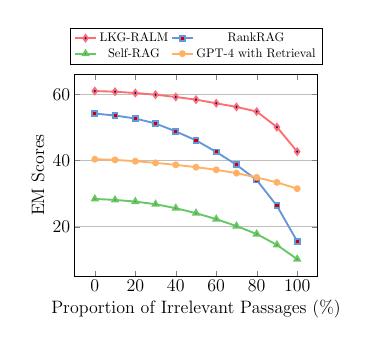
\begin{tikzpicture}[scale=0.45]
    \begin{axis}[
        xlabel=Proportion of Irrelevant Passages (\%),
        ylabel=EM Scores,
        % y label style={at={(-0.0,0.5)}},
        ymajorgrids=true,
        font=\Large,
        legend style={at={(0.5,1.05)}, anchor=south, legend columns=2, draw=black, fill=white,align=left,font=\normalsize},
    ]
        \addplot+[color={rgb,255:red,255;green,110;blue,110}, line width=1.5pt, mark=diamond*, mark size=2.5pt] coordinates {
            (0,61.0)
            (10,60.8)
            (20,60.4)
            (30,59.9)
            (40,59.2)
            (50,58.4)
            (60,57.3)
            (70,56.2)
            (80,54.8)
            (90,50.1)
            (100,42.7)
        };
        \addlegendentry{LKG-RALM};
        \addplot+[color={rgb,255:red,100;green,150;blue,220}, line width=1.5pt, mark=square*, mark size=2pt] coordinates {
            (0,54.2)
            (10,53.6)
            (20,52.7)
            (30,51.2)
            (40,48.8)
            (50,46.1)
            (60,42.6)
            (70,38.7)
            (80,34.1)
            (90,26.3)
            (100,15.6)
        };
        \addlegendentry{RankRAG};
        \addplot+[color={rgb,255:red,100;green,200;blue,100}, line width=1.5pt, mark=triangle*, mark size=2.5pt] coordinates {
            (0,28.4)
            (10,28.1)
            (20,27.6)
            (30,26.8)
            (40,25.6)
            (50,24.1)
            (60,22.3)
            (70,20.2)
            (80,17.8)
            (90,14.5)
            (100,10.2)
        };
        \addlegendentry{Self-RAG};
        \addplot+[color=orange!60, line width=1.5pt, mark=*, mark size=2pt] coordinates {
            (0,40.4)
            (10,40.2)
            (20,39.8)
            (30,39.3)
            (40,38.7)
            (50,38.0)
            (60,37.2)
            (70,36.2)
            (80,34.9)
            (90,33.4)
            (100,31.5)
        };
        \addlegendentry{GPT-4 with Retrieval};
    \end{axis}
\end{tikzpicture}
\label{fig:q4-2}
\end{minipage}
}
\caption{Robustness to the number of retrieved passages and the proportion of irrelevant passages.}
\label{fig:impact_passages}
\end{figure}
Our method internally attends attention to relevant passages for the given question, facilitating evidence-seeking from noisy contexts. To evaluate its robustness and noise tolerance, we conducted adversarial testing by incrementally replacing the 50 retrieved passages with irrelevant passages, ranging from 0\% to 100\% substitution.

From Figure \ref{fig:q4-2}, LKG-RALM showed strong resilience against irrelevant information. When increasing irrelevant passages to 100\%, the EM score only gradually decreased from 61.0 to 42.7, significantly outperforming other retrieval-based models. Even with 80\% irrelevant input, LKG-RALM maintained a strong EM score of 54.8. In comparison, models without explicit relevance modeling like RankRAG saw sharp performance drops, falling from 54.2 to 15.6 with fully irrelevant passages. While GPT-4 with Retrieval showed high noise tolerance, dropping only from 40.4 to 31.5 under fully irrelevant conditions, it did not leverage relevant information as effectively as LKG-RALM, as shown in our earlier experiment. LKG-RALM's superior performance stems from its explicit relevance modeling, which helps it focus on pertinent information while filtering out noise. This allows it to effectively balance the use of retrieved knowledge with its inherent model capabilities.


% From Figure \ref{fig:q4-2}, we observed that LKG-RALM demonstrated remarkable resilience to noise and irrelevant information. As the proportion of irrelevant passages increased to 100\%, the EM score exhibited only a gradual decline from 61.0 to 42.7, significantly outpacing other retrieval-based models under similar conditions. Even when 80\% of the input was irrelevant, LKG-RALM maintained a high EM score of 54.8. In contrast, models lacking explicit relevance modeling, such as RankRAG, experienced substantial performance degradation, dropping from 54.2 to 15.6 under fully irrelevant conditions. GPT-4 with Retrieval showed the highest robustness to irrelevant passages, with its performance only marginally decreasing from 40.4 to 31.5 under fully irrelevant conditions. However, it did not fully utilize additional relevant information as effectively as LKG-RALM, as seen in the first experiment. The superior performance of LKG-RALM can be attributed to its explicit relevance modeling, enabling it to focus on pertinent passages while effectively ignoring distractions in extremely noisy environments. By leveraging its well-trained parametric knowledge and external information effectively, LKG-RALM strikes an optimal balance between utilizing retrieved knowledge and relying on inherent model capabilities.



% \begin{figure}[t]
\centering
\begin{minipage}[t]{1\linewidth}
\centering
\includegraphics[width=1.0\textwidth]{figure/src/attention_visual.pdf}
\end{minipage}
\centering
\caption{The visualization of QPI's attention weights in HC-LLM, where the heatmap shows the attention weights between questions and passages across model layers. The x-axis corresponds to the passages and question serving as attention keys/values, while the y-axis indexes the HC-LLM layers. A darker color indicates a larger attention weight. In this case, $p_5$ and $p_{13}$ contain answer evidence and receive higher weighting, while the irrelevant passages receive lower attention weights. This demonstrates how the question-guided focusing helps identify and prioritize the most relevant contexts for answering.}
\label{fig:visual}
\end{figure}
% \subsection{(Q5) Visual Analysis}
% % 不同attention层的可视化效果,参考ROME论文,看attention权重找文章准不准,对比相关性添加前后的可视化效果
% To offer transparent insights into the inner workings of the HC-LLM architecture, we conduct explanatory visual analysis investigating the cross-attention distributions modeled within the Question-Passage Interaction component. Specifically, we analyze the impact of incorporating supervised question-passage relevance on steering the model's evidence extraction towards pertinent passages.

% In the default setting without explicit relevance modeling, the attention weights are dispersed across all input passages regardless of pertinence. However, after integrating relevance supervision that imparts physical interpretation to the attention distributions, we observe a gradual concentration of the attention weights towards key evidence-bearing passages across layers, effectively filtering out distracting irrelevant ones. For example in Figure \ref{fig:visual}, the relevance-incorporated attention heatmap clearly illustrates shrinking weights allocation on non-critical passages. Meanwhile, passages containing answer-bearing evidence receive concentrated attention. This validates that the relevance modeling successfully provides effective top-down guidance for HC-LLM to focus on salient passages and mitigate noise interference.

% Remarkably, we also notice substantial attention retained on the question itself in deeper layers. This intriguing phenomenon suggests that without useful evidence contexts, HC-LLM can still leverage its internal pre-trained knowledge and reasoning strength to deeply comprehend the question semantics. It can then generate answers by exploiting the parametric connections between query concepts and world knowledge within the foundation language model. Such intrinsic capability offers fail-safe robustness against absent or noisy passages. Overall, these visualizations offer explanatory power regarding how the relevance mechanism interacts with pre-trained knowledge to facilitate noise-resilient evidence extraction for ODQA.

\section{Conclusion}
In this work, we proposed LKG-RALM, which leverages layer-wise knowledge within LLMs to guide attention toward relevant passages, addressing distractibility and positional bias in handling retrieved passages. A layer-wise passage estimator evaluates passage relevance by utilizing diverse layer knowledge within the LLM. Entropy-based layer-knowledge selection dynamically identifies the most relevant layers for accurate passage assessment. Relevance-aware passage fusion selectively prioritizes crucial content, reducing the impact of irrelevant passages and overcoming positional bias. Extensive experiments across multiple datasets demonstrate that LKG-RALM achieves notable improvements in accuracy and robustness for knowledge-intensive tasks.

\section*{Limitations}
Our work has several important limitations that should be acknowledged:

First, while our layer-wise passage estimator significantly improves RALM performance, it introduces additional computational overhead. The need to process passages through multiple layers for relevance assessment increases both memory usage and inference time. Although this overhead is relatively small compared to the base LLM inference, it may impact real-time applications or resource-constrained environments. Future work could explore more efficient methods for leveraging layer-wise knowledge without significant computational costs.

Second, our approach relies heavily on the quality of retrieved passages. While LKG-RALM shows improved robustness to irrelevant passages, its performance still degrades when the retrieval quality is poor or when dealing with queries requiring information beyond the knowledge cutoff date of the retrieval corpus. This limitation is particularly evident in rapidly evolving domains where the retrieved information may become outdated quickly.

Third, the effectiveness of our layer-knowledge selection mechanism may vary across different LLM architectures and sizes. While we demonstrated strong performance with LLAMA-3.1 and Qwen-2.5, the optimal configuration of layer-wise knowledge utilization might need to be adjusted for different model architectures. Additionally, our current approach to entropy-based layer selection may not capture all aspects of layer-specific knowledge representation.

\section*{Ethics Statement}
Our work utilizes publicly available datasets and pre-trained language models, adhering to established data usage guidelines. However, several ethical considerations deserve attention. While LKG-RALM shows improved robustness in handling retrieved information, it inherits potential biases present in both the pre-trained language models and the retrieval corpus, which could affect the model's responses across different demographic groups or topic areas. We emphasize that our work primarily focuses on technical improvements in retrieval-augmented language modeling and should be complemented with dedicated bias mitigation strategies. Additionally, the improved performance of our model in handling retrieved passages raises questions about information authenticity and attribution. While LKG-RALM can better identify and utilize relevant information, users should be aware that the model's responses are based on retrieved passages that may contain inaccuracies or outdated information. We recommend implementing clear attribution mechanisms and confidence indicators in practical applications.

\section*{Acknowledgments}
This work is supported by the National Natural Science Foundation of China (Grant No. 62102277), the National Key R\&D Program of China under Grant No. 2022YFC3303600, the Zhejiang Provincial Natural Science Foundation of China under Grant No. LY23F020010.

\bibliography{custom}

\appendix

\section{Attention Analysis Setting} \label{Attention pattern analysis}
\subsection{Model and Dataset Selection}
Our analysis of attention patterns in Retrieval-Augmented Language Models (RALMs) was conducted using LLAMA-3.1-8B-instruct as the base model. We randomly selected a sample of 2000 queries from the Natural Questions and TraviaQA datasets, which consist of real-world queries submitted to Google Search and Allen Institute along with high-quality human-annotated answers extracted from Wikipedia pages.

\subsection{Attention Pattern Classification}
In our study, we focused on three main categories of attention patterns: edge-focused attention, uniform attention, and middle-focused attention. To analyze these patterns, we examined the attention distribution across all attention heads in the model. For each attention head, we calculated the percentage of attention allocated to different parts of the input sequence, specifically the beginning, middle, and end. Based on this distribution, we classified each attention head into one of the three main categories. We then quantified the prevalence of each attention pattern type across all attention heads to gain a comprehensive understanding of the model's attention behavior.

\subsection{Correlation Analysis}
To investigate the relationship between attention patterns and model performance, we conducted a correlation analysis. This involved calculating the sum of attention weights for each pattern type and measuring the model's accuracy on the test set. We then computed the correlation between these attention weight sums and the model's accuracy for each pattern type. This analysis allowed us to identify which attention patterns were most strongly associated with improved model performance.

\subsection{Manipulation Experiments}
To further validate our findings and explore the causal relationships between attention patterns and model performance, we conducted two types of manipulation experiments. In the first experiment, we artificially replaced edge-focused and uniform attention patterns with middle-focused attention on relevant passages. This allowed us to observe how redirecting attention to potentially more informative parts of the input affected the model's performance. In the second experiment, we deliberately redirected middle-focused attention patterns to both irrelevant and relevant passages. By comparing the model's performance under these different conditions, we were able to assess the impact of focused attention on specific parts of the input.

Throughout our analysis, we created detailed visualizations to illustrate the different attention patterns and their impact on model performance. These visualizations, presented in Figure \ref{fig:attention pattern} and Figure \ref{fig:attention replacement}, provide a clear and intuitive representation of our findings, helping to elucidate the complex relationships between attention mechanisms and RALM performance. By systematically examining different types of attention patterns, their prevalence, and their relationship to model accuracy, we have identified potential areas for improvement in model design and training, particularly in guiding attention to relevant parts of the input for enhanced performance in open-domain question answering tasks.

\section{Dataset Description} \label{dataset description}
To comprehensively evaluate the performance of Retrieval-Augmented Language Models (RALMs) across diverse data characteristics, we employ a range of representative datasets covering various aspects of question-answering tasks, from factoid questions to multi-hop reasoning and strategy-based inquiries. Below, we provide detailed descriptions of each dataset:

\begin{itemize}
    \item \textit{Natural Questions (NQ)}: Developed by Google Research \cite{NQ}, this dataset comprises real-world queries submitted to Google Search, accompanied by high-quality human-annotated answers extracted from Wikipedia pages. NQ offers a rich mixture of long and short answer formats, reflecting authentic information-seeking behaviors across a broad range of subjects. Its structure, featuring both comprehensive passages and concise answer spans, provides a nuanced testing ground for RALMs.
    \item \textit{TriviaQA}: Crafted by researchers at the Allen Institute for AI \cite{TQA}, TriviaQA presents a formidable challenge with its extensive collection of question-answer pairs. These are sourced from trivia enthusiasts and paired with supporting evidence from Wikipedia and web searches. The dataset's hallmark is its high lexical and syntactic variance between questions and answers, necessitating robust retrieval and reasoning capabilities from models. By spanning both web and Wikipedia domains, it offers a comprehensive evaluation landscape.
    \item \textit{StrategyQA}: Developed by the Allen Institute for AI \cite{strategyQA}, it focuses on multi-hop reasoning questions that demand implicit strategic thinking. StrategyQA's questions often require common sense reasoning, with answers typically being binary (yes/no) but necessitating complex cognitive processes. It is specifically designed to challenge and evaluate models' strategic thinking abilities, pushing the boundaries of AI reasoning.
    \item \textit{HotpotQA}: A collaborative effort by Carnegie Mellon University \cite{HotpotQA}, HotpotQA features Wikipedia-based question-answer pairs that explicitly require reasoning across multiple supporting documents. It includes sentence-level supporting facts for answer explanation and maintains a balance across different reasoning types, such as bridging and comparison. This structure makes HotpotQA particularly effective in assessing multi-hop reasoning capabilities.
    \item \textit{PopQA}: Created by researchers at the University of Washington \cite{PopQA}, PopQA centers on questions about popular culture, including movies, music, celebrities, and current events. This dataset is crucial for testing models' ability to handle contemporary and rapidly evolving information. It challenges RALMs to navigate ambiguity and context-dependent information, reflecting the dynamic nature of real-world knowledge.
    \item \textit{2WikiMQA}: Developed by the Graduate University for Advanced Studies \cite{ho2020constructing}, 2WikiMQA is a multi-hop open-domain question-answering dataset constructed from Wikipedia. It features questions that necessitate reasoning across multiple Wikipedia pages and includes complex queries that cannot be answered by a single fact. This dataset is designed to simultaneously test both retrieval accuracy and advanced reasoning capabilities of RALMs.
\end{itemize}

By employing this diverse set of benchmarks, we aim to provide a holistic assessment of model capabilities, from factual recall to complex reasoning and strategic thinking. 

\section{Baseline Settings} \label{baseline setting}
Our baseline methods for open-QA tasks represent a diverse range of approaches, from pure language models to sophisticated retrieval-augmented systems. We categorize these baselines into three groups: closed-book LLM without retrieval, LLM with retrieval, and robust RALM. Each group showcases different strategies for tackling RAG challenges.

\subsection{Closed-book LLM without retrieval and LLM with retrieval}
The first two groups encompass state-of-the-art language models that have demonstrated exceptional capabilities in various natural language processing tasks. For models in the LLM with retrieval category, we employ a straightforward approach of concatenating retrieved content to the context, allowing the LLM to process the augmented input:
\begin{itemize}
    \item \textit{LLAMA-3.1} (2024) \cite{dubey2024llama}: The latest iteration in the LLaMA series, LLAMA-3.1 builds upon 15 trillion texts, achieving the most effective open-source ability.
    \item \textit{Qwen-2.5} (2024) \cite{yang2024qwen2}: Developed by Alibaba, Qwen-2.5 represents a significant advancement in multilingual capabilities, trained on 18 trillion data to achieve state-of-the-art performance across various tasks.
    \item \textit{ChatGPT} (2022): Developed by OpenAI, this model has gained widespread recognition for its conversational prowess and extensive knowledge base across diverse domains.
    \item \textit{GPT-4} (2023) \cite{gpt4}: A large-scale, multimodal model developed by OpenAI, capable of accepting image and text inputs and producing text outputs. It exhibits human-level performance on various professional and academic benchmarks.
    \item \textit{Claude-3-Sonnet} (2024): An advanced AI model from Anthropic, part of the Claude 3 model family, known for its strong performance across a wide range of tasks.
\end{itemize}

\subsection{Robust RALM}
The third group comprises advanced retrieval-augmented language models that enhance the robustness and effectiveness of RAG:
\begin{itemize}
    \item \textit{REPLUG} (2023) \cite{REPLUG}: A retrieval-augmented language modeling framework that treats the language model as a black box and augments it with a tuneable retrieval model. It simply prepends retrieved documents to the input for the frozen black-box LM.
    \item \textit{Self-RAG} (2023) \cite{asai2023self}: A framework that enhances an LM's quality and factuality through retrieval and self-reflection. It trains a single arbitrary LM that adaptively retrieves passages on-demand, and generates and reflects on retrieved passages and its own generations using special tokens.
    \item \textit{RA-ISF} (2024) \cite{liu2024ra}: A framework that iteratively decomposes tasks and processes them in three submodules to enhance the model's problem-solving capabilities. It aims to improve factual reasoning capabilities and reduce hallucinations.
    \item \textit{Noise-Resistant RALM} (2024) \cite{yoran2024making}: This approach focuses on making retrieval-augmented language models robust to irrelevant context. It proposes two methods: a simple baseline that filters out retrieved passages using an NLI model, and a method for automatically generating data to fine-tune the language model.
    \item \textit{ChatQA-1.5} (2024) \cite{liu2024chatqa}: An evolution of the ChatQA model, this version introduces refinements aimed at enhancing effectiveness in question-answering tasks, particularly in conversational contexts.
    \item \textit{RankRAG} (2024) \cite{yu2024rankrag}: A instruction fine-tuning framework that instruction-tunes a single LLM for the dual purpose of context ranking and answer generation in RAG.
\end{itemize}

In our experimental setup, the RankRAG results are referenced from the original paper using LLaMA-3-70B in a zero-shot setting and are supported by the authors; ChatQA \footnote{https://huggingface.co/nvidia/Llama3-ChatQA-1.5-70B} leverages LLaMA-3-70B in a five-shot setting; Noise-Resistant RALM \footnote{https://huggingface.co/datasets/Ori/strategyqa-ret-robust} is reproduced using LLaMA-3.1-8B; and RA-ISF \footnote{https://github.com/OceannTwT/ra-isf} is implemented with ChatGPT-3.5.

\section{Implementation Details}
Our model foundation utilizes LLAMA and Qwen. For retrieval, we follow ATLAS \cite{atlas} by using the Wikipedia dump from December 20, 2018, as our external corpus, comprising 28 million passages. We adopt a hybrid retrieval \cite{arivazhagan2023hybrid}, where BM25 is grounded on the Elastic Search \cite{es}, while the dense retriever is based on the FAISS index \cite{FAISS}. The training data is followed by Self-RAG \cite{asai2023self}. The trainable low-rank weights were implemented using LoRA \cite{hu2021lora}, with a rank dimension of 256. The hidden size of the adaptor is set to 4096. We optimized all trainable parameters using the AdamW optimizer with a learning rate of 1e-5. The batch size was set to 32, and a warmup ratio of 0.1 was employed along with a cosine learning rate scheduler. Three external relevance scores are obtained from BGE-M3 \footnote{https://huggingface.co/BAAI/bge-m3}, E5-mistral-7b-instruct \footnote{https://huggingface.co/intfloat/e5-mistral-7b-instruct}, GTE-Qwen2-7B-instruct \footnote{https://huggingface.co/Alibaba-NLP/gte-Qwen2-7B-instruct}. The updating factor $\beta$ for layer-wised relevance guidance was set to 0.2. 

Notice that we can use separate LLMs for passage estimation and answer generation in parallel. A lighter estimator (e.g., 1.5B) paired with a larger generator (e.g., 8B) minimizes overhead, where the generator can share relevance guidance across some layers due to differing layer counts.

For the attention pattern analysis, we define the first 3 tokens as the head and the last 3 tokens as the tail, with the remaining tokens classified as the middle. We employ threshold-based metrics to distinguish between attention patterns:
\begin{itemize}
    \item Edge-focused: Combined attention weights of head and tail exceed 75\%.
    \item Uniform: Middle attention weights exceed 90\%, with over 40\% of tokens having attention weights greater than 1/(input length), and no single token's attention weight exceeding 10\%. The term "uniform" is somewhat hyperbolic. What it actually represents is a pattern where no single token receives exceptionally high attention. 
    \item Middle-focused: Middle attention weights exceed 90\%, with either one or two tokens having attention weights above 30\%, or three or more tokens having attention weights above 10\%.
\end{itemize}


\section{Performance on general NLP tasks}
Beyond open-QA, we assess the capabilities of LKG-RALM architecture on broader NLP benchmarks. Specifically, we evaluate on Multitask Language Understanding (MMLU) and Language Modeling, standing challenging tasks covering both understanding and generation.

\subsection{MMLU}
\begin{table}[t]
\footnotesize
\begin{center}
\begin{tabular}{llccccc} 
\hline
\textbf{Model} &  \textbf{Hum.} & \textbf{Social.} & \textbf{STEM} & \textbf{Other} & \textbf{All} \\
\hline
LLAMA-3-8B  & 73.8 & 75.2 & 69.5 & 73.5 & 73.0 \\
ChatGPT  & 71.2 & 73.6 & 65.8 & 69.4 & 70.0 \\
GPT4  & 85.7 & 87.9 & 84.2 & 87.8 & 86.4 \\
Self-RAG  & 64.5 & 65.8 & 63.1 & 65.4 & 64.7 \\
RankRAG  & 74.1 & 75.6 & 70.8 & 73.5 & 73.5 \\
\hline
LKG-RALM-8B  & 75.3 & 77.2 & 71.9 & 74.8 & 74.8 \\
\hline
\end{tabular}
\end{center}
\caption{Performance on MMLU task.}
\label{table:MMLU}
\end{table}
We evaluated LKG-RALM on the Multi-task Language Understanding (MMLU) benchmark \cite{mmlu}, a comprehensive multiple choice QA dataset consisting of 57 natural language understanding tasks, including elementary mathematics, US history, computer science, law, and more. Following previous work \cite{REPLUG}, We grouped these tasks into four categories: Humanities, Social Science, STEM, and Other. We still use the Wikipedia dump as an external corpus for retrieving information to improve the performance on the MMLU task.


As shown in Table \ref{table:MMLU}, the results demonstrate that LKG-RALM outperforms the original LLAMA model by a significant margin across all tasks. Specifically, we observe an average accuracy improvement of 1.5\% on Humanities, 7.2\% on Social Science, 2.8\% on STEM, and 4.4\% on other tasks over LLAMA-3.1-8B. Moreover, compared to other models, we have achieved competitive performance. LKG-RALM-8B outperforms ChatGPT by 4.8\% on average and surpasses Self-RAG by 10.1\%. Compared with RankRAG, we obtain 1.3 absolute improvements on average. This substantial performance boost can be attributed to two key factors. Firstly, the retrieved passages from Wikipedia provide useful external knowledge and context for the model to better understand the input texts. Secondly, the relevance-guided architecture enables more effective encoding and reasoning over lengthy context-like passages, facilitating passage understanding for solving complex MMLU tasks.

\subsection{Language Modeling}
\setlength{\tabcolsep}{1.5pt}  % 默认值是6pt
\begin{table}[t]
\footnotesize
\begin{center}
\begin{tabular}{llccc} 
\hline
\textbf{Model} & \textbf{\# Params} & \textbf{Original} & \textbf{+LKG-RALM} & \textbf{Gain \%}\\
\hline
\multirow{4}*{GPT-2} & 117M & 1.33 & 1.22 & 8.27 \\
 & 345M & 1.20 & 1.13 & 10.83 \\
 & 774M & 1.19 & 1.14 & 4.20 \\
 & 1.5B & 1.16 & 1.01 & 12.93 \\
\hline
\multirow{3}*{Qwen-2.5} & 7B & 0.95 & 0.90 & 5.26 \\
& 14B & 0.88 & 0.84 & 4.54 \\
& 72B & 0.70 & 0.66 & 5.71 \\
\hline
\multirow{2}*{LLAMA-3.1} & 8B & 0.97 & 0.93 & 4.12 \\
 & 70B & 0.72 & 0.70 & 2.77 \\
\hline
\end{tabular}
\end{center}
\caption{Performance on language modeling task}
\label{table:LM}
\end{table}

As a crucial touchstone for evaluating general language generation capabilities, we assess the LKG-RALM architecture on language modeling benchmarks spanning diverse domains including websites, academic writing, code, and dialogue on the Pile dataset. These benchmarks require predicting subsequent tokens based on preceding textual context, and evaluating model fluency, coherence and grounding. A key challenge arises from lengthy context segmentation across long documents, which hinders encoding the full history to produce logically consistent continuations. To enable relevance-aware passage fusion component, we segment lengthy sequences into 100-token passages. 

Following prior work \cite{REPLUG}, we report the standard bits-per-byte (BPB) metric which measures cross-entropy reduction to evaluate perplexity improvements. A smaller value of BPB means better performance. As shown in Table \ref{table:LM}, LKG-RALM substantially enhances base LLMs like GPT-2, Qwen, and LLAMA across all categories of the Pile benchmark by 9.06\% (GPT-2), 5.17\% (Qwen), and 3.45\% (LLAMA) BPB on average. This demonstrates LKG-RALM successfully encodes rich multi-granularity semantics to produce logical and human-like text continuations. The significant perplexity reductions validate that hierarchical encoding mechanisms enhance the language model's context capacity to track lengthy precedings for coherent generation. By effectively navigating long-range dependencies, LKG-RALM generates higher-quality and better-grounded natural language.

\section{Efficiency and Accuracy Trade-off}
\begin{table}[t]
\footnotesize
\begin{center}
\caption{Efficiency and Accuracy Trade-off for LKG-RALM and Baseline Models under 1024 Context Tokens.}
\begin{tabular}{lccc}
\hline
\textbf{Model} & \textbf{EM} & \textbf{Speed (s/query)} & \textbf{TFLOPs} \\
\hline
Self-RAG & 28.4 & 3.07 & 20.5 \\
RA-ISF & 31.3 & 3.44 & 63.8 \\
Robust-RALM & 45.7 & 0.74 & 14.6 \\
RankRAG & 54.2 & 1.25 & 145.4 \\
\hline
\multicolumn{4}{c}{\textbf{LKG-RALM with Different Passage Estimator}} \\
\hline
LLAMA-3.1-8B & 30.9 & 0.82 & 16.3 \\
\hspace{0.1cm} + Qwen-2.5-500M & 53.6 & 0.83 & 18.1 \\
\hspace{0.1cm} + Qwen-2.5-1.5B & 54.8 & 0.85 & 20.0 \\
\hspace{0.1cm} + Qwen-2.5-7B   & 55.3 & 0.91 & 30.9 \\
\hline
LLAMA-3.1-70B & 42.7 & 1.24 & 142.6 \\
\hspace{0.1cm} + Qwen-2.5-500M & 60.0 & 1.24 & 144.4 \\
\hspace{0.1cm} + Qwen-2.5-1.5B & 60.7 & 1.25 & 146.3 \\
\hspace{0.1cm} + Qwen-2.5-7B   & 61.0 & 1.27 & 157.2 \\
\hline
\end{tabular}
\label{table:efficiency-accuracy}
\end{center}
\end{table}

To contextualize our method's efficiency, we compared LKG-RALM's performance with existing models in Table \ref{table:efficiency-accuracy}. Self-RAG and RA-ISF require multiple rounds of retrieval and question decomposition-based multi-turn dialogue, respectively. Their low parallelism results in approximately 3.7x inference time compared to LLAMA-3.1-8B, with Self-RAG taking 3.07 seconds per query and RA-ISF requiring 3.44 seconds per query. Noise-Resistant-8B and RankRAG-70B use BERT-based NLI models and Reranking Models, respectively, to assist in passage filtering or sorting. This introduces an additional 0.8\% inference latency and 1.9\% computational overhead for RankRAG-70B, increasing its processing time to 1.25 seconds per query and its computational cost to 145.4 TFLOPs for 1024 tokens. Similarly, LKG-RALM-70B employs the Qwen-2.5-7B model for passage relevance analysis, resulting in a 2.4\% increase in inference latency (from 1.24 to 1.27 s/query) and a 10.2\% increase in computational cost (from 142.6 to 157.2 TFLOPs). The low latency is attributed to the layer-wise passage estimator's ability to operate in high parallelism with LLM inference.

To further evaluate the trade-off between efficiency and accuracy, we conducted experiments using different LLM sizes for the layer-wise passage estimator. Table \ref{table:efficiency-accuracy} shows that increasing the size of the passage estimator from Qwen-2.5-500M to Qwen-2.5-7B yields consistent improvements in EM scores for both LLAMA-3.1-8B and LLAMA-3.1-70B base models. For LLAMA-3.1-8B, the EM score improves from 53.6 to 55.3 as we scale up the estimator, with a modest increase in processing time from 0.83 to 0.91 seconds per query. The computational cost rises from 18.1 to 30.9 TFLOPs. Notably, even with the largest Qwen-2.5-7B estimator, LKG-RALM-70B maintains competitive efficiency compared to RankRAG-70B (1.27 vs 1.25 s/query) while achieving superior EM scores (61.0 vs 54.2). LKG-RALM's flexible framework allows users to balance accuracy and efficiency by selecting appropriate estimator sizes. For example, Qwen-2.5-1.5B with LLAMA-3.1-70B improves EM score by 0.7 over the 500M version, with minimal increases in query time and computational cost.

\section{Effects of Training Data Size}
\begin{figure}[t]
\centering
\subfigure[NQ]{
\begin{minipage}[t]{0.46\linewidth}
\centering
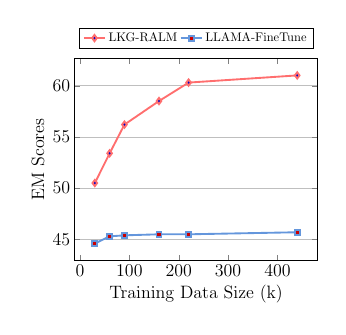
\begin{tikzpicture}[scale=0.45]
    \begin{axis}[
        xlabel=Training Data Size (k),
        ylabel=EM Scores,
        % y label style={at={(-0.0,0.5)}},
        ymajorgrids=true,
        font=\Large,
        legend style={at={(0.5,1.05)}, anchor=south, legend columns=2, draw=black, fill=white,align=left,font=\normalsize},
    ]
        \addplot+[color={rgb,255:red,255;green,110;blue,110}, line width=1.5pt, mark=diamond*, mark size=2.5pt] coordinates {
            (30,50.5)
            (60,53.4)
            (90,56.2)
            (160,58.5)
            (220,60.3)
            (440,61.0)
        };
        \addlegendentry{LKG-RALM};
        \addplot+[color={rgb,255:red,100;green,150;blue,220}, line width=1.5pt, mark=square*, mark size=2pt] coordinates {
            (30,44.6)
            (60,45.3)
            (90,45.4)
            (160,45.5)
            (220,45.5)
            (440,45.7)
        };
        \addlegendentry{LLAMA-FineTune};
    \end{axis}
\end{tikzpicture}
\label{fig:nq-data-size}
\end{minipage}
}
\hfill
\subfigure[HotpotQA]{
\begin{minipage}[t]{0.46\linewidth}
\centering
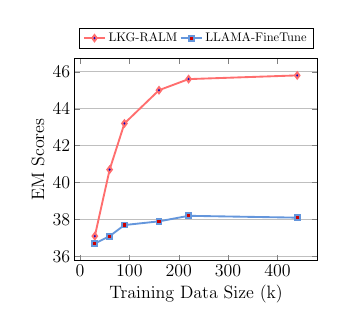
\begin{tikzpicture}[scale=0.45]
    \begin{axis}[
        xlabel=Training Data Size (k),
        ylabel=EM Scores,
        % y label style={at={(-0.0,0.5)}},
        ymajorgrids=true,
        font=\Large,
        legend style={at={(0.5,1.05)}, anchor=south, legend columns=2, draw=black, fill=white,align=left,font=\normalsize},
    ]
        \addplot+[color={rgb,255:red,255;green,110;blue,110}, line width=1.5pt, mark=diamond*, mark size=2.5pt] coordinates {
            (30,37.1)
            (60,40.7)
            (90,43.2)
            (160,45.0)
            (220,45.6)
            (440,45.8)
        };
        \addlegendentry{LKG-RALM};
        \addplot+[color={rgb,255:red,100;green,150;blue,220}, line width=1.5pt, mark=square*, mark size=2pt] coordinates {
            (30,36.7)
            (60,37.1)
            (90,37.7)
            (160,37.9)
            (220,38.2)
            (440,38.1)
        };
        \addlegendentry{LLAMA-FineTune};
    \end{axis}
\end{tikzpicture}
\label{fig:hotpotqa-data-size}
\end{minipage}
}
\caption{Effects of training data size.}
\label{fig:data-size-impact}
\end{figure}
We conducted an analysis to understand how the scale of training data affects the model's performance. Specifically, we randomly sampled 30k, 60k, 90k, 160k, and 220k instances from our original 440k training instances and fine-tuned five LKG-RALM-70B variants on these subsets. We then compared the model performance on NQ and HotpotQA with our final LKG-RALM trained on the full 440k instances. We also evaluated LLAMA-3.1-70B fine-tuned on the same data subsets as a baseline. Figure \ref{fig:data-size-impact} shows the models' performance trained on different amounts of data. For NQ, LKG-RALM-70B's accuracy improves from 50.5 with 30k training instances to 61.0 with the full 440k dataset. In contrast, LLAMA-3.1-FineTune shows minimal improvement, from 44.6 to 45.7 with a mere 1.1 increase. The performance gap between LKG-RALM-70B and LLAMA-3.1-FineTune widens significantly, from 5.9 at 30k instances to 15.3 at 440k instances. 

The model's strong performance largely comes from its effective pre-training parameter space. With only 30k fine-tuning examples, LKG-RALM-70B shows impressive results, reaching 50.5 EM on NQ and 37.1 on HotpotQA. This indicates that minimal fine-tuning data can activate the model's core capabilities in passage estimation and robustness. The performance difference between LKG-RALM-70B and LLAMA-3.1-FineTune is clear even with limited data, showing our approach's effectiveness. As training data increases, LKG-RALM-70B's accuracy steadily improves, though gains slow after 220k examples. For NQ, the improvement from 220k to 440k is just 0.7, versus 1.8 from 160k to 220k. This shows that while more data helps performance, the benefits decrease with larger datasets. The model's architecture and pre-training are key to its success, enabling strong results with limited fine-tuning data, while additional training data has diminishing returns.

\section{Impact of Relevance Score Quantity}
To investigate how the number of relevance scores affects model performance, we conducted experiments that preserved only the first k distinct relevance scores (k ranging from 1 to 7). Any subsequent relevance scores that were either similar or appeared later in the sequence were overwritten by these values. In our analysis of a 32-layer LLMAMA-3.1-8B, we observed significantly different relevance scores (L1 distance >0.3) distributed across layers. The distribution of these distinct scores is presented in Table \ref{tab:score-distribution}.

\setlength{\tabcolsep}{4pt}  % 默认值是6pt
\begin{table}[t]
\scriptsize
\centering
\caption{Distribution of Distinct Relevance Scores Across Model Layers}
\label{tab:score-distribution}
\begin{tabular}{lcccccccc}
\hline
Number of Scores & 1 & 2 & 3 & 4 & 5 & 6 & 7 & Others \\
\hline
Percentage (\%) & 4.2 & 17.2 & 21.8 & 35.9 & 10.4 & 5.6 & 3.2 & 1.7 \\
\hline
\end{tabular}
\end{table}

\setlength{\tabcolsep}{3pt}  % 默认值是6pt
\begin{table}[t]
\scriptsize
\centering
\caption{Model Performance with Different Numbers of Relevance Scores}
\label{tab:score-impact}
\begin{tabular}{lccccc}
\hline
Model & NQ & TriviaQA & HotpotQA & PopQA & 2WikiMQA \\
\hline
LLAMA-3.1-8B & 18.7 & 78.5 & 16.5 & 22.1 & 13.9 \\
+ Retrieval \& Fine-tuning & 35.7 & 77.4 & 28.9 & 37.1 & 25.3 \\
\hline
+ LKG-RALM (k=1) & 36.4 & 77.3 & 29.6 & 38.6 & 26.2 \\
+ LKG-RALM (k=2) & 40.7 & 78.5 & 31.3 & 42.3 & 26.5 \\
+ LKG-RALM (k=3) & 47.2 & 85.4 & 37.4 & 48.0 & 33.4 \\
+ LKG-RALM (k=4) & 50.1 & 86.0 & 39.3 & 51.6 & 34.6 \\
+ LKG-RALM (k=5) & 51.6 & 86.0 & 40.5 & 52.3 & 35.0 \\
+ LKG-RALM (k=6) & 51.9 & 86.1 & 40.5 & 53.2 & 35.4 \\
+ LKG-RALM (k=7) & 51.8 & 86.2 & 40.1 & 53.3 & 35.5 \\
+ LKG-RALM (all) & 55.3 & 88.6 & 43.1 & 57.2 & 39.0 \\
\hline
\end{tabular}
\end{table}

The impact of varying k values on model performance across different datasets is shown in Table \ref{tab:score-impact}. The result reveals that LKG-RALM's accuracy consistently improved across metrics as more relevance scores were incorporated into the attention guidance mechanism. Notably significant performance improvements were observed at several key transitions. When increasing from k=2 to k=3, we observed substantial gains across all datasets, with NQ accuracy improving by 6.5 points (from 40.7 to 47.2) and TriviaQA showing a remarkable 6.9-point increase (from 78.5 to 85.4). The transition from k=3 to k=4 brought further improvements, particularly in NQ (2.9 points) and PopQA (3.6 points). Interestingly, while incremental improvements continued beyond k=4, they became more modest, with gains typically under 1.5 points per step.

The most striking performance boost was achieved when utilizing all relevance scores instead of limiting to the first seven distinct scores. This configuration led to substantial improvements across all datasets: NQ improved by 3.5 points (from 51.8 to 55.3), TriviaQA by 2.4 points (from 86.2 to 88.6), and 2WikiMQA by 3.5 points (from 35.5 to 39.0). These results strongly suggest that while the first few distinct relevance scores contribute significantly to model performance, the additional nuanced guidance from higher layers plays a crucial role in maximizing the model's capabilities.

While our experimental design focused on retaining the first k relevance scores, this approach may not be optimal as higher-layer knowledge representations could provide essential guidance for complex reasoning tasks. The superior performance achieved when utilizing all attention guidance signals validates their collective importance in enhancing model accuracy and demonstrates the value of maintaining a diverse set of relevance scores across different layers of the model architecture.



\end{document}
